% --- IMPORTS ---
\documentclass[leqno]{article}
\usepackage{graphicx}
\usepackage{dsfont}
\usepackage{mathtools}
\usepackage{amssymb}
\usepackage{amsmath}
\usepackage{amsthm}
\usepackage{float}
\usepackage{ragged2e}
\usepackage{tensor}
\usepackage{fancyhdr}
\usepackage{empheq}
\usepackage[most]{tcolorbox}
\usepackage{enumitem}
\usepackage{dirtytalk}
\usepackage{marginnote}
\usepackage{microtype}
\usepackage[
  a4paper,
  left=0.8in,
  right=1in,
  top=1in,
  bottom=0.5in,
  headheight=14pt,
  headsep=0.4in
]{geometry}
\setlength{\parindent}{0cm}
% --- TikZ Packages ---
\usepackage{pgfplots}
\pgfplotsset{compat=1.18}
\usepgfplotslibrary{fillbetween, polar}
\usetikzlibrary{calc, positioning}
\usetikzlibrary{angles, quotes}
\usetikzlibrary{arrows.meta}
\usetikzlibrary{decorations.pathreplacing, decorations.markings}
\usetikzlibrary{patterns}
\usetikzlibrary{intersections}
% --- URL Packages ---
\usepackage[colorlinks=true,linkcolor=red,citecolor=magenta,urlcolor=black]{hyperref}%
\urlstyle{same}
% --- END OF IMPORTS ---

% --- CUSTOM COMMANDS ---
\RenewDocumentCommand{\marks}{o m}{%
  \IfValueTF{#1}%
    {\marginnote{\raggedright\textbf{[#2]}}[#1]}%
    {\marginnote{\raggedright\textbf{[#2]}}}%
}
\newcommand{\vspacerule}[2]{%
  \par\vspace*{#1}%
  \noindent\hrulefill\par
  \vspace*{#2}%
}
\definecolor{scarlet}{RGB}{205, 40, 75}
\newcommand{\questionitem}{%
  \item\phantomsection
  \addcontentsline{toc}{section}{Question \number\value{enumi}}%
}
\renewcommand{\contentsname}{Questions}
% --- END OF CUSTOM COMMANDS ---

% --- HEADER CONFIG ---
\pagestyle{fancy}
\fancyhead{}
\fancyfoot{}
\renewcommand{\headrulewidth}{0.9pt}
\lhead{\textit{Solutions} - De Moivre's Theorem}
\chead{}
\rhead{\href{https://danieljsmith.org}{danieljsmith.org}}
% --- END OF HEADER CONFIG ---

\begin{document}
\vspace*{20pt}
\tableofcontents
\newpage
\begin{enumerate}[
  label=\textbf{\arabic*.},
  leftmargin=*,
  topsep=0pt,
  partopsep=0pt,
  parsep=0pt
]

% ---- Question 1 ----
\questionitem

A complex number $z$ has modulus $1$ and argument $\theta$. \\
\begin{enumerate}[label=\textbf{(\alph*)}]
  \item Show that
  \[
  z^n + \frac{1}{z^n} = 2\cos n\theta
  \quad\text{and}\quad
  z^n - \frac{1}{z^n} = 2\mathrm{i}\sin n\theta,
  \qquad n \in \mathbb{Z}^+
  \]
  \marks[-20pt]{3}
  \item Hence, by expanding $\left(z + \frac{1}{z}\right)^3$ and $\left(z - \frac{1}{z}\right)^3$, show that
  \[
  \tan 3\theta = \frac{3\tan\theta - \tan^3\theta}{1 - 3\tan^2\theta}
  \]
  \marks[-20pt]{4}
\end{enumerate}

\vspace*{10pt}

\begin{tcolorbox}[colback=white, colframe=scarlet, title={\textbf{Solution}}, breakable, grow to left by=6mm, grow to right by=10mm]
\begin{enumerate}[label=\textbf{(\alph*)}]
  \item Since $|z|=1$ and $\arg z=\theta$,
\[
z=\cos\theta+\mathrm{i}\sin\theta=e^{\mathrm{i}\theta}
\]
So, by De Moivre's theorem,
\[
z^n=e^{\mathrm{i}n\theta}=\cos n\theta+\mathrm{i}\sin n\theta
\]
Also,
\[
\frac{1}{z}=e^{-\mathrm{i}\theta}
\]
and hence
\[
\frac{1}{z^n}=e^{-\mathrm{i}n\theta}=\cos n\theta-\mathrm{i}\sin n\theta
\]

Now add:
\[
z^n+\frac{1}{z^n}
=(\cos n\theta+\mathrm{i}\sin n\theta)+(\cos n\theta-\mathrm{i}\sin n\theta)
=2\cos n\theta
\]

Now subtract:
\[
z^n-\frac{1}{z^n}
=(\cos n\theta+\mathrm{i}\sin n\theta)-(\cos n\theta-\mathrm{i}\sin n\theta)
=2\mathrm{i}\sin n\theta
\]

Therefore
\[
z^n+\frac{1}{z^n}=2\cos n\theta
\quad\text{and}\quad
z^n-\frac{1}{z^n}=2\mathrm{i}\sin n\theta
\]

  \item From part (a), with $n=1$,
\[
z+\frac{1}{z}=2\cos\theta
\]
Cubing both sides gives
\[
\left(z+\frac{1}{z}\right)^3=(2\cos\theta)^3=8\cos^3\theta
\]

Expand the left-hand side:
\begin{align*}
\left(z+\frac{1}{z}\right)^3
&=z^3+3z+\frac{3}{z}+\frac{1}{z^3} \\
&=\left(z^3+\frac{1}{z^3}\right)+3\left(z+\frac{1}{z}\right)
\end{align*}
Using part (a) again,
\[
8\cos^3\theta=2\cos3\theta+6\cos\theta
\]
So
\[
\cos3\theta=4\cos^3\theta-3\cos\theta
\]

Now use part (a) with
\[
z-\frac{1}{z}=2\mathrm{i}\sin\theta
\]
Cubing both sides,
\[
\left(z-\frac{1}{z}\right)^3=(2\mathrm{i}\sin\theta)^3=-8\mathrm{i}\sin^3\theta
\]

Expand:
\begin{align*}
\left(z-\frac{1}{z}\right)^3
&=z^3-3z+\frac{3}{z}-\frac{1}{z^3} \\
&=\left(z^3-\frac{1}{z^3}\right)-3\left(z-\frac{1}{z}\right)
\end{align*}
Using part (a),
\[
-8\mathrm{i}\sin^3\theta=2\mathrm{i}\sin3\theta-6\mathrm{i}\sin\theta
\]
Hence
\[
\sin3\theta=3\sin\theta-4\sin^3\theta
\]

Let $t=\tan\theta$. Then
\begin{align*}
\tan3\theta
&=\frac{\sin3\theta}{\cos3\theta} \\[5pt]
&=\frac{\dfrac{\sin3\theta}{\cos^3\theta}}{\dfrac{\cos3\theta}{\cos^3\theta}} \\[5pt]
&=\frac{\dfrac{3\sin\theta-4\sin^3\theta}{\cos^3\theta}}{\dfrac{4\cos^3\theta-3\cos\theta}{\cos^3\theta}} \\[5pt]
&=\frac{3\tan\theta\sec^2\theta-4\tan^3\theta}{4-3\sec^2\theta} \\[5pt]
&=\frac{3t(1+t^2)-4t^3}{4-3(1+t^2)} \\[5pt]
&=\frac{3t-t^3}{1-3t^2}
\end{align*}
Therefore
\[
\tan3\theta=\frac{3\tan\theta-\tan^3\theta}{1-3\tan^2\theta}
\]
\end{enumerate}
\end{tcolorbox}


\newpage

% ---- Question 2 ----
\questionitem

\begin{enumerate}[label=\textbf{(\alph*)}]
  \item Using de Moivre's theorem, show that
  \[
  \sin^4\theta\cos^2\theta \equiv \frac{1}{32}(\cos 6\theta - 2\cos 4\theta - \cos 2\theta + 2)
  \]
  \marks[-20pt]{5}
  \item By using the substitution $\alpha=\left(\frac{\pi}{2}-\theta\right)$, or otherwise, find a similar identity for $\sin^2\theta\cos^4\theta$. \marks{3} \\
  \item Given that $0<a<\frac{\pi}{2}$ and
  \[
  \int_0^a \left(\sin^4\theta\cos^2\theta + 2\sin^2\theta\cos^4\theta\right)\,\mathrm{d}\theta = \frac{\pi}{32} - \frac{\sqrt{3}}{64}
  \]
  find the exact value of $a$. \marks{5} \\
\end{enumerate}

\vspace*{10pt}

\begin{tcolorbox}[colback=white, colframe=scarlet, title={\textbf{Solution}}, breakable, grow to left by=6mm, grow to right by=10mm]
\begin{enumerate}[label=\textbf{(\alph*)}]
\item Let
\[
c=\cos 2\theta
\]

Using the double-angle identities,
\[
\sin^2\theta=\frac{1-\cos 2\theta}{2}=\frac{1-c}{2},
\qquad
\cos^2\theta=\frac{1+\cos 2\theta}{2}=\frac{1+c}{2}
\]

So
\begin{align*}
\sin^4\theta\cos^2\theta
&=\left(\frac{1-c}{2}\right)^2\left(\frac{1+c}{2}\right) \\
&=\frac18(1-2c+c^2)(1+c) \\
&=\frac18(1+c-2c-2c^2+c^2+c^3) \\
&=\frac18(1-c-c^2+c^3)
\end{align*}

Now use de Moivre's theorem.

From
\[
(\cos 2\theta+\mathrm{i}\sin 2\theta)^2=\cos 4\theta+\mathrm{i}\sin 4\theta
\]
taking real parts gives
\[
\cos 4\theta=2\cos^2 2\theta-1=2c^2-1
\]
so
\[
c^2=\frac{1+\cos 4\theta}{2}
\]

Also, from
\[
(\cos 2\theta+\mathrm{i}\sin 2\theta)^3=\cos 6\theta+\mathrm{i}\sin 6\theta
\]
taking real parts gives
\[
\cos 6\theta=4\cos^3 2\theta-3\cos 2\theta=4c^3-3c
\]
so
\[
c^3=\frac{\cos 6\theta+3c}{4}
\]

Substituting these into \(\frac18(1-c-c^2+c^3)\),
\begin{align*}
\sin^4\theta\cos^2\theta
&=\frac18\left(1-c-\frac{1+\cos 4\theta}{2}+\frac{\cos 6\theta+3c}{4}\right) \\
&=\frac18\left(\frac{4-4c-2-2\cos 4\theta+\cos 6\theta+3c}{4}\right) \\
&=\frac{1}{32}\left(2-c-2\cos 4\theta+\cos 6\theta\right)
\end{align*}

Since \(c=\cos 2\theta\),
\[
\sin^4\theta\cos^2\theta\equiv \frac{1}{32}\left(\cos 6\theta-2\cos 4\theta-\cos 2\theta+2\right)
\]

Hence the required identity is shown.

\item Let
\[
\alpha=\frac{\pi}{2}-\theta
\]

Then
\[
\sin\theta=\cos\alpha,
\qquad
\cos\theta=\sin\alpha
\]
so
\[
\sin^2\theta\cos^4\theta=\cos^2\alpha\sin^4\alpha=\sin^4\alpha\cos^2\alpha
\]

Using part (a),
\[
\sin^4\alpha\cos^2\alpha=\frac{1}{32}\left(\cos 6\alpha-2\cos 4\alpha-\cos 2\alpha+2\right)
\]

Now
\[
2\alpha=\pi-2\theta,\quad 4\alpha=2\pi-4\theta,\quad 6\alpha=3\pi-6\theta
\]
so
\[
\cos 2\alpha=-\cos 2\theta,\qquad \cos 4\alpha=\cos 4\theta,\qquad \cos 6\alpha=-\cos 6\theta
\]

Therefore
\[
\sin^2\theta\cos^4\theta
=\frac{1}{32}\left(-\cos 6\theta-2\cos 4\theta+\cos 2\theta+2\right)
\]

So a similar identity is
\[
\sin^2\theta\cos^4\theta\equiv \frac{1}{32}\left(-\cos 6\theta-2\cos 4\theta+\cos 2\theta+2\right)
\]

\item Let
\[
I(a)=\int_0^a\left(\sin^4\theta\cos^2\theta+2\sin^2\theta\cos^4\theta\right)\,\mathrm{d}\theta
\]

Using parts (a) and (b),
\begin{align*}
\sin^4\theta\cos^2\theta+2\sin^2\theta\cos^4\theta
&=\frac{1}{32}\left(\cos 6\theta-2\cos 4\theta-\cos 2\theta+2\right) \\
&\quad +\frac{2}{32}\left(-\cos 6\theta-2\cos 4\theta+\cos 2\theta+2\right) \\
&=\frac{1}{32}\left(-\cos 6\theta-6\cos 4\theta+\cos 2\theta+6\right)
\end{align*}

Hence
\begin{align*}
I(a)
&=\frac{1}{32}\int_0^a\left(-\cos 6\theta-6\cos 4\theta+\cos 2\theta+6\right)\,\mathrm{d}\theta \\
&=\frac{1}{32}\left[-\frac16\sin 6\theta-\frac32\sin 4\theta+\frac12\sin 2\theta+6\theta\right]_0^a \\
&=\frac{1}{32}\left(6a+\frac12\sin 2a-\frac32\sin 4a-\frac16\sin 6a\right)
\end{align*}

We are given that
\[
I(a)=\frac{\pi}{32}-\frac{\sqrt3}{64}
\]

Try \(a=\frac{\pi}{6}\). Then
\[
6a=\pi,\qquad \sin 2a=\sin\frac{\pi}{3}=\frac{\sqrt3}{2},\qquad
\sin 4a=\sin\frac{2\pi}{3}=\frac{\sqrt3}{2},\qquad
\sin 6a=\sin\pi=0
\]

So
\begin{align*}
I\left(\frac{\pi}{6}\right)
&=\frac{1}{32}\left(\pi+\frac12\cdot\frac{\sqrt3}{2}-\frac32\cdot\frac{\sqrt3}{2}-0\right) \\
&=\frac{1}{32}\left(\pi-\frac{\sqrt3}{2}\right) \\
&=\frac{\pi}{32}-\frac{\sqrt3}{64}
\end{align*}

So \(a=\frac{\pi}{6}\) satisfies the equation.

To show this is the only solution, differentiate \(I(a)\) using the Fundamental Theorem of Calculus:
\[
I'(a)=\sin^4 a\cos^2 a+2\sin^2 a\cos^4 a
\]
and factorise:
\[
I'(a)=\sin^2 a\cos^2 a(\sin^2 a+2\cos^2 a)
\]

For \(0<a<\frac{\pi}{2}\), we have \(\sin a>0\) and \(\cos a>0\), so
\[
I'(a)>0
\]
Thus \(I(a)\) is strictly increasing on \(\left(0,\frac{\pi}{2}\right)\), so the solution is unique.

Therefore
\[
a=\frac{\pi}{6}
\]
that is, \(a=30^\circ\).
\end{enumerate}
\end{tcolorbox}


\newpage

% ---- Question 3 ----
\questionitem

Use de Moivre's theorem to find the constants $A$, $B$ and $C$ in the identity
\[
\sin\theta\cos^4\theta = A\sin\theta + B\sin 3\theta + C\sin 5\theta
\]
\marks[-20pt]{4}

\vspace*{10pt}

\begin{tcolorbox}[colback=white, colframe=scarlet, title={\textbf{Solution}}, breakable, grow to left by=6mm, grow to right by=10mm]
Let
\[
z=\cos\theta+\mathrm{i}\sin\theta
\]
Then \(z^{-1}=\cos\theta-\mathrm{i}\sin\theta\), so
\[
\cos\theta=\frac{z+z^{-1}}{2},
\qquad
\sin\theta=\frac{z-z^{-1}}{2\mathrm{i}}
\]
Also, by de Moivre's theorem,
\[
z^n=\cos n\theta+\mathrm{i}\sin n\theta
\]
which gives
\[
\sin n\theta=\frac{z^n-z^{-n}}{2\mathrm{i}}
\]

Now write \(\sin\theta\cos^4\theta\) in terms of \(z\):

\begin{align*}
\sin\theta\cos^4\theta
&=\frac{z-z^{-1}}{2\mathrm{i}}\left(\frac{z+z^{-1}}{2}\right)^4 \\
&=\frac{1}{32\mathrm{i}}(z-z^{-1})(z+z^{-1})^4
\end{align*}

Expand \((z+z^{-1})^4\):

\[
(z+z^{-1})^4=z^4+4z^2+6+4z^{-2}+z^{-4}
\]

So

\begin{align*}
\sin\theta\cos^4\theta
&=\frac{1}{32\mathrm{i}}(z-z^{-1})(z^4+4z^2+6+4z^{-2}+z^{-4}) \\
&=\frac{1}{32\mathrm{i}}\bigl(z^5+4z^3+6z+4z^{-1}+z^{-3} \\
&\qquad\qquad\qquad {}-z^3-4z-6z^{-1}-4z^{-3}-z^{-5}\bigr) \\
&=\frac{1}{32\mathrm{i}}\bigl(z^5+3z^3+2z-2z^{-1}-3z^{-3}-z^{-5}\bigr) \\
&=\frac{1}{32\mathrm{i}}\Bigl[(z^5-z^{-5})+3(z^3-z^{-3})+2(z-z^{-1})\Bigr]
\end{align*}

Now use
\[
\frac{z^n-z^{-n}}{2\mathrm{i}}=\sin n\theta
\]

Hence

\begin{align*}
\sin\theta\cos^4\theta
&=\frac{1}{16}\sin5\theta+\frac{3}{16}\sin3\theta+\frac{2}{16}\sin\theta \\
&=\frac{1}{8}\sin\theta+\frac{3}{16}\sin3\theta+\frac{1}{16}\sin5\theta
\end{align*}

Comparing with
\[
\sin\theta\cos^4\theta=A\sin\theta+B\sin3\theta+C\sin5\theta
\]
gives
\[
A=\frac{1}{8},\qquad B=\frac{3}{16},\qquad C=\frac{1}{16}
\]
\end{tcolorbox}


\newpage

% ---- Question 4 ----
\questionitem

\begin{enumerate}[label=\textbf{(\roman*)}]
  \item Starting with the result
  \[
  e^{\mathrm{i}\theta}=\cos\theta+\mathrm{i}\sin\theta
  \]
  show that
  \begin{enumerate}[label=(\Alph*)]
    \item
    \[
    \left(\cos\theta+\mathrm{i}\sin\theta\right)^n=\cos n\theta+\mathrm{i}\sin n\theta
    \]
    \marks[-20pt]{2}
    \item
    \[
    \sin\theta=\frac{1}{2\mathrm{i}}\left(e^{\mathrm{i}\theta}-e^{-\mathrm{i}\theta}\right)
    \]
    \marks[-20pt]{2}
  \end{enumerate}
  \item Using the result in part (i)(A), obtain the values of the constants $a$, $b$, $c$, $d$ and $e$ in the identity
  \[
  \cos 8\theta \equiv a\sin^8\theta+b\sin^6\theta+c\sin^4\theta+d\sin^2\theta+e
  \]
  \marks[-20pt]{6}
  \item Using the result in part (i)(B), obtain the values of the constants $P$, $Q$, $R$, $S$ and $T$ in the identity
  \[
  \sin^8\theta \equiv P\cos 8\theta+Q\cos 6\theta+R\cos 4\theta+S\cos 2\theta+T
  \]
  \marks[-20pt]{6}
  \item Hence show that
  \[
  \sin \frac{\pi}{8}=\left(\frac{17-12\sqrt{2}}{64}\right)^{\frac{1}{8}}
  \]
  \marks[-20pt]{3}
\end{enumerate}

\vspace*{10pt}

\begin{tcolorbox}[colback=white, colframe=scarlet, title={\textbf{Solution}}, breakable, grow to left by=6mm, grow to right by=10mm]
\begin{enumerate}[label=\textbf{(\roman*)}]
  \item
  \begin{enumerate}[label=\textbf{(\Alph*)}]
    \item Starting from
    \[
    e^{\mathrm{i}\theta}=\cos\theta+\mathrm{i}\sin\theta
    \]
    raise both sides to the power \(n\):
    \[
    \left(\cos\theta+\mathrm{i}\sin\theta\right)^n=\left(e^{\mathrm{i}\theta}\right)^n=e^{\mathrm{i}n\theta}
    \]
    Now apply Euler's formula again, with \(\theta\) replaced by \(n\theta\):
    \[
    e^{\mathrm{i}n\theta}=\cos n\theta+\mathrm{i}\sin n\theta
    \]
    Hence
    \[
    \left(\cos\theta+\mathrm{i}\sin\theta\right)^n=\cos n\theta+\mathrm{i}\sin n\theta
    \]

    \item Replace \(\theta\) by \(-\theta\) in Euler's formula:
    \[
    e^{-\mathrm{i}\theta}=\cos(-\theta)+\mathrm{i}\sin(-\theta)=\cos\theta-\mathrm{i}\sin\theta
    \]
    Subtract this from
    \[
    e^{\mathrm{i}\theta}=\cos\theta+\mathrm{i}\sin\theta
    \]
    to get
    \[
    e^{\mathrm{i}\theta}-e^{-\mathrm{i}\theta}=2\mathrm{i}\sin\theta
    \]
    Therefore
    \[
    \sin\theta=\frac{1}{2\mathrm{i}}\left(e^{\mathrm{i}\theta}-e^{-\mathrm{i}\theta}\right)
    \]
  \end{enumerate}

  \item Let \(C=\cos\theta\) and \(S=\sin\theta\). From part \textbf{(i)(A)},
  \[
  (C+\mathrm{i}S)^8=\cos 8\theta+\mathrm{i}\sin 8\theta
  \]
  Expand \((C+\mathrm{i}S)^8\):
  \begin{align*}
  (C+\mathrm{i}S)^8
  &=C^8+8\mathrm{i}C^7S+28C^6(\mathrm{i}S)^2+56C^5(\mathrm{i}S)^3+70C^4(\mathrm{i}S)^4 \\
  &\qquad +56C^3(\mathrm{i}S)^5+28C^2(\mathrm{i}S)^6+8C(\mathrm{i}S)^7+(\mathrm{i}S)^8 \\
  &=C^8+8\mathrm{i}C^7S-28C^6S^2-56\mathrm{i}C^5S^3+70C^4S^4 \\
  &\qquad +56\mathrm{i}C^3S^5-28C^2S^6-8\mathrm{i}CS^7+S^8
  \end{align*}
  Taking real parts,
  \[
  \cos 8\theta=C^8-28C^6S^2+70C^4S^4-28C^2S^6+S^8
  \]
  Since \(C^2=1-S^2\), let \(x=S^2\). Then
  \begin{align*}
  \cos 8\theta
  &=(1-x)^4-28(1-x)^3x+70(1-x)^2x^2-28(1-x)x^3+x^4 \\
  &=(1-4x+6x^2-4x^3+x^4) \\
  &\qquad -28(x-3x^2+3x^3-x^4) \\
  &\qquad +70(x^2-2x^3+x^4)-28(x^3-x^4)+x^4 \\
  &=1-32x+160x^2-256x^3+128x^4
  \end{align*}
  Substitute back \(x=\sin^2\theta\):
  \[
  \cos 8\theta \equiv 128\sin^8\theta-256\sin^6\theta+160\sin^4\theta-32\sin^2\theta+1
  \]
  Hence
  \[
  a=128,\quad b=-256,\quad c=160,\quad d=-32,\quad e=1
  \]

  \item From part \textbf{(i)(B)},
  \[
  \sin\theta=\frac{1}{2\mathrm{i}}\left(e^{\mathrm{i}\theta}-e^{-\mathrm{i}\theta}\right)
  \]
  Therefore
  \[
  \sin^8\theta=\left(\frac{1}{2\mathrm{i}}\right)^8\left(e^{\mathrm{i}\theta}-e^{-\mathrm{i}\theta}\right)^8
  =\frac{1}{256}\left(e^{\mathrm{i}\theta}-e^{-\mathrm{i}\theta}\right)^8
  \]
  Now expand:
  \begin{align*}
  \sin^8\theta
  &=\frac{1}{256}\Bigl(
  e^{8\mathrm{i}\theta}-8e^{6\mathrm{i}\theta}+28e^{4\mathrm{i}\theta}-56e^{2\mathrm{i}\theta}+70 \\
  &\qquad\qquad\qquad -56e^{-2\mathrm{i}\theta}+28e^{-4\mathrm{i}\theta}-8e^{-6\mathrm{i}\theta}+e^{-8\mathrm{i}\theta}
  \Bigr)
  \end{align*}
  Use
  \[
  e^{k\mathrm{i}\theta}+e^{-k\mathrm{i}\theta}=2\cos k\theta
  \]
  so that
  \begin{align*}
  \sin^8\theta
  &=\frac{1}{256}\Bigl(
  (e^{8\mathrm{i}\theta}+e^{-8\mathrm{i}\theta})
  -8(e^{6\mathrm{i}\theta}+e^{-6\mathrm{i}\theta}) \\
  &\qquad\qquad
  +28(e^{4\mathrm{i}\theta}+e^{-4\mathrm{i}\theta})
  -56(e^{2\mathrm{i}\theta}+e^{-2\mathrm{i}\theta})
  +70
  \Bigr) \\
  &=\frac{1}{256}\Bigl(
  2\cos 8\theta-16\cos 6\theta+56\cos 4\theta-112\cos 2\theta+70
  \Bigr) \\
  &=\frac{1}{128}\cos 8\theta-\frac{1}{16}\cos 6\theta+\frac{7}{32}\cos 4\theta-\frac{7}{16}\cos 2\theta+\frac{35}{128}
  \end{align*}
  So
  \[
  P=\frac{1}{128},\quad Q=-\frac{1}{16},\quad R=\frac{7}{32},\quad S=-\frac{7}{16},\quad T=\frac{35}{128}
  \]
  Equivalently,
  \[
  \sin^8\theta\equiv \frac{\cos 8\theta-8\cos 6\theta+28\cos 4\theta-56\cos 2\theta+35}{128}
  \]

  \item Using the identity from part \textbf{(iii)} with \(\theta=\dfrac{\pi}{8}\),
  \[
  \sin^8\frac{\pi}{8}
  =\frac{\cos\pi-8\cos\frac{3\pi}{4}+28\cos\frac{\pi}{2}-56\cos\frac{\pi}{4}+35}{128}
  \]
  Now
  \[
  \cos\pi=-1,\qquad \cos\frac{3\pi}{4}=-\frac{\sqrt2}{2},\qquad \cos\frac{\pi}{2}=0,\qquad \cos\frac{\pi}{4}=\frac{\sqrt2}{2}
  \]
  so
  \begin{align*}
  \sin^8\frac{\pi}{8}
  &=\frac{-1-8\left(-\frac{\sqrt2}{2}\right)+28(0)-56\left(\frac{\sqrt2}{2}\right)+35}{128} \\
  &=\frac{-1+4\sqrt2-28\sqrt2+35}{128} \\
  &=\frac{34-24\sqrt2}{128} \\
  &=\frac{17-12\sqrt2}{64}
  \end{align*}
  Since \(0<\dfrac{\pi}{8}<\dfrac{\pi}{2}\), \(\sin\dfrac{\pi}{8}>0\). Hence
  \[
  \sin \frac{\pi}{8}=\left(\frac{17-12\sqrt{2}}{64}\right)^{\frac{1}{8}}
  \]
\end{enumerate}
\end{tcolorbox}


\newpage

% ---- Question 5 ----
\questionitem

\begin{enumerate}[label=\textbf{(\alph*)}]
  \item Use de Moivre's theorem to show that $\cos 6\theta \equiv (1 - 2\sin^2\theta)(16\sin^4\theta - 16\sin^2\theta + 1)$ \marks{5} \\
  \item By solving the equation $\cos 6\theta = 0$, deduce that $\sin^2\left(\frac{\pi}{12}\right) = \frac{2 - \sqrt{3}}{4}$. \marks{4} \\
  \item Hence, or otherwise, write down the exact values of $\sin^2\left(\frac{5\pi}{12}\right)$, $\sin^2\left(\frac{7\pi}{12}\right)$ and $\sin^2\left(\frac{11\pi}{12}\right)$. \marks{3} \\
\end{enumerate}

\vspace*{10pt}

\begin{tcolorbox}[colback=white, colframe=scarlet, title={\textbf{Solution}}, breakable, grow to left by=6mm, grow to right by=10mm]
\begin{enumerate}[label=\textbf{(\alph*)}]
  \item Using de Moivre's theorem,
\[
(\cos\theta+\mathrm{i}\sin\theta)^6=\cos6\theta+\mathrm{i}\sin6\theta
\]

Expand the left-hand side by the binomial theorem:
\begin{align*}
(\cos\theta+\mathrm{i}\sin\theta)^6
&=\cos^6\theta+6\cos^5\theta(\mathrm{i}\sin\theta)+15\cos^4\theta(\mathrm{i}\sin\theta)^2 \\
&\quad +20\cos^3\theta(\mathrm{i}\sin\theta)^3+15\cos^2\theta(\mathrm{i}\sin\theta)^4 \\
&\quad +6\cos\theta(\mathrm{i}\sin\theta)^5+(\mathrm{i}\sin\theta)^6 \\
&=\cos^6\theta+6\mathrm{i}\cos^5\theta\sin\theta-15\cos^4\theta\sin^2\theta \\
&\quad -20\mathrm{i}\cos^3\theta\sin^3\theta+15\cos^2\theta\sin^4\theta \\
&\quad +6\mathrm{i}\cos\theta\sin^5\theta-\sin^6\theta
\end{align*}

Taking real parts gives
\[
\cos6\theta=\cos^6\theta-15\cos^4\theta\sin^2\theta+15\cos^2\theta\sin^4\theta-\sin^6\theta
\]

Now let
\[
u=\sin^2\theta
\qquad \text{so} \qquad
\cos^2\theta=1-u
\]

Then
\begin{align*}
\cos6\theta
&=(1-u)^3-15(1-u)^2u+15(1-u)u^2-u^3 \\
&=(1-3u+3u^2-u^3)-15(u-2u^2+u^3)+15(u^2-u^3)-u^3 \\
&=1-3u+3u^2-u^3-15u+30u^2-15u^3+15u^2-15u^3-u^3 \\
&=1-18u+48u^2-32u^3
\end{align*}

Now factorise:
\begin{align*}
1-18u+48u^2-32u^3
&=(1-2u)(16u^2-16u+1)
\end{align*}

Substituting back \(u=\sin^2\theta\),
\[
\cos6\theta=(1-2\sin^2\theta)(16\sin^4\theta-16\sin^2\theta+1)
\]

Hence
\[
\cos 6\theta \equiv (1 - 2\sin^2\theta)(16\sin^4\theta - 16\sin^2\theta + 1)
\]

  \item Let
\[
u=\sin^2\theta
\]

From part (a), if \(\cos6\theta=0\), then
\[
(1-2u)(16u^2-16u+1)=0
\]

So either
\[
1-2u=0 \quad \Rightarrow \quad u=\frac12
\]
or
\begin{align*}
16u^2-16u+1&=0 \\
u&=\frac{16\pm\sqrt{(-16)^2-4(16)(1)}}{2\cdot16} \\
&=\frac{16\pm\sqrt{256-64}}{32} \\
&=\frac{16\pm\sqrt{192}}{32} \\
&=\frac{16\pm8\sqrt3}{32} \\
&=\frac{2\pm\sqrt3}{4}
\end{align*}

Now
\[
\cos\left(6\cdot\frac{\pi}{12}\right)=\cos\frac{\pi}{2}=0
\]
so \(\sin^2\left(\frac{\pi}{12}\right)\) must be one of
\[
\frac12,\quad \frac{2+\sqrt3}{4},\quad \frac{2-\sqrt3}{4}
\]

But
\[
0<\frac{\pi}{12}<\frac{\pi}{4}
\]
so
\[
\sin^2\left(\frac{\pi}{12}\right)<\sin^2\left(\frac{\pi}{4}\right)=\frac12
\]

Therefore the correct value is
\[
\sin^2\left(\frac{\pi}{12}\right)=\frac{2-\sqrt3}{4}
\]

  \item Using part (b),
\begin{align*}
\sin^2\left(\frac{5\pi}{12}\right)
&=\cos^2\left(\frac{\pi}{12}\right) \\
&=1-\sin^2\left(\frac{\pi}{12}\right) \\
&=1-\frac{2-\sqrt3}{4} \\
&=\frac{2+\sqrt3}{4}
\end{align*}

Also,
\[
\sin^2\left(\frac{7\pi}{12}\right)=\sin^2\left(\pi-\frac{5\pi}{12}\right)=\sin^2\left(\frac{5\pi}{12}\right)=\frac{2+\sqrt3}{4}
\]

and
\[
\sin^2\left(\frac{11\pi}{12}\right)=\sin^2\left(\pi-\frac{\pi}{12}\right)=\sin^2\left(\frac{\pi}{12}\right)=\frac{2-\sqrt3}{4}
\]

Hence
\[
\sin^2\left(\frac{5\pi}{12}\right)=\frac{2+\sqrt3}{4},\qquad
\sin^2\left(\frac{7\pi}{12}\right)=\frac{2+\sqrt3}{4},\qquad
\sin^2\left(\frac{11\pi}{12}\right)=\frac{2-\sqrt3}{4}
\]
\end{enumerate}
\end{tcolorbox}


\newpage

% ---- Question 6 ----
\questionitem

Let $t=\tan\theta$. By writing
\[
\cos\theta+\mathrm{i}\sin\theta=\cos\theta\,(1+\mathrm{i}t)
\]
and expanding $(1+\mathrm{i}t)^6$, use de Moivre's theorem to show that
\[
\tan 6\theta=\frac{6\tan\theta-20\tan^3\theta+6\tan^5\theta}{1-15\tan^2\theta+15\tan^4\theta-\tan^6\theta}
\]
\marks[-30pt]{7}

\vspace*{10pt}

\begin{tcolorbox}[colback=white, colframe=scarlet, title={\textbf{Solution}}, breakable, grow to left by=6mm, grow to right by=10mm]
Let
\[
z=\cos\theta+\mathrm{i}\sin\theta
\]
and let
\[
t=\tan\theta=\frac{\sin\theta}{\cos\theta}
\]

Then \(\sin\theta=t\cos\theta\), so
\[
z=\cos\theta+\mathrm{i}\sin\theta=\cos\theta+\mathrm{i}(t\cos\theta)=\cos\theta(1+\mathrm{i}t)
\]

Now apply de Moivre's theorem:
\[
z^6=\cos 6\theta+\mathrm{i}\sin 6\theta
\]

But also, from \(z=\cos\theta(1+\mathrm{i}t)\),
\[
z^6=\cos^6\theta\,(1+\mathrm{i}t)^6
\]

So we expand \((1+\mathrm{i}t)^6\) using the binomial theorem:
\[
(1+\mathrm{i}t)^6
=1+6(\mathrm{i}t)+15(\mathrm{i}t)^2+20(\mathrm{i}t)^3+15(\mathrm{i}t)^4+6(\mathrm{i}t)^5+(\mathrm{i}t)^6
\]

Now simplify the powers of \(\mathrm{i}\):
\[
\mathrm{i}^2=-1,\qquad \mathrm{i}^3=-\mathrm{i},\qquad \mathrm{i}^4=1,\qquad \mathrm{i}^5=\mathrm{i},\qquad \mathrm{i}^6=-1
\]

Hence
\begin{align*}
(1+\mathrm{i}t)^6
&=1+6\mathrm{i}t+15(-1)t^2+20(-\mathrm{i})t^3+15(1)t^4+6(\mathrm{i})t^5+(-1)t^6 \\
&=1+6\mathrm{i}t-15t^2-20\mathrm{i}t^3+15t^4+6\mathrm{i}t^5-t^6 \\
&=(1-15t^2+15t^4-t^6)+\mathrm{i}(6t-20t^3+6t^5)
\end{align*}

Therefore
\begin{align*}
\cos 6\theta+\mathrm{i}\sin 6\theta
&=\cos^6\theta\Bigl[(1-15t^2+15t^4-t^6)+\mathrm{i}(6t-20t^3+6t^5)\Bigr]
\end{align*}

Equating real and imaginary parts gives
\[
\cos 6\theta=\cos^6\theta(1-15t^2+15t^4-t^6)
\]
and
\[
\sin 6\theta=\cos^6\theta(6t-20t^3+6t^5)
\]

So
\begin{align*}
\tan 6\theta
&=\frac{\sin 6\theta}{\cos 6\theta} \\
&=\frac{\cos^6\theta(6t-20t^3+6t^5)}{\cos^6\theta(1-15t^2+15t^4-t^6)} \\
&=\frac{6t-20t^3+6t^5}{1-15t^2+15t^4-t^6}
\end{align*}

Since \(t=\tan\theta\), this becomes
\[
\tan 6\theta=\frac{6\tan\theta-20\tan^3\theta+6\tan^5\theta}{1-15\tan^2\theta+15\tan^4\theta-\tan^6\theta}
\]

which is the required result.
\end{tcolorbox}


\newpage

% ---- Question 7 ----
\questionitem

\begin{enumerate}[label=\textbf{(\alph*)}]
  \item Use de Moivre's theorem to show that
  \[
  \sin 6x = \sin 2x\left(a\cos^4 x + b\cos^2 x + c\right)
  \]
  where $a$, $b$ and $c$ are integers to be determined. \marks{4} \\
  \item Hence solve, for $0<\theta<\frac{\pi}{2}$,
  \[
  \sin 6\theta = \sin 2\theta \cos 2\theta
  \]
  giving your answers to $3$ decimal places. \marks{4} \\
\end{enumerate}

\vspace*{10pt}

\begin{tcolorbox}[colback=white, colframe=scarlet, title={\textbf{Solution}}, breakable, grow to left by=6mm, grow to right by=10mm]
\begin{enumerate}[label=\textbf{(\alph*)}]
  \item Let $C=\cos x$ and $S=\sin x$.

By de Moivre's theorem,
\[
(\cos x+\mathrm{i}\sin x)^6=\cos 6x+\mathrm{i}\sin 6x
\]

So
\begin{align*}
(C+\mathrm{i}S)^6
&=C^6+6\mathrm{i}C^5S+15C^4(\mathrm{i}S)^2+20C^3(\mathrm{i}S)^3+15C^2(\mathrm{i}S)^4+6C(\mathrm{i}S)^5+(\mathrm{i}S)^6 \\
&=C^6+6\mathrm{i}C^5S-15C^4S^2-20\mathrm{i}C^3S^3+15C^2S^4+6\mathrm{i}CS^5-S^6
\end{align*}

Taking imaginary parts gives
\begin{align*}
\sin 6x
&=6C^5S-20C^3S^3+6CS^5 \\
&=2CS\left(3C^4-10C^2S^2+3S^4\right)
\end{align*}

Now simplify the bracket:
\begin{align*}
3C^4-10C^2S^2+3S^4
&=3(C^4+S^4)-10C^2S^2 \\
&=3\bigl((C^2+S^2)^2-2C^2S^2\bigr)-10C^2S^2 \\
&=3(1-2C^2S^2)-10C^2S^2 \\
&=3-16C^2S^2 \\
&=3-16C^2(1-C^2) \\
&=16C^4-16C^2+3
\end{align*}

Also, $\sin 2x=2\sin x\cos x=2CS$, so
\[
\sin 6x=\sin 2x\left(16\cos^4x-16\cos^2x+3\right)
\]

Hence
\[
a=16,\qquad b=-16,\qquad c=3
\]

  \item Using part (a),
\[
\sin 6\theta=\sin 2\theta\left(16\cos^4\theta-16\cos^2\theta+3\right)
\]

So the equation
\[
\sin 6\theta=\sin 2\theta\cos 2\theta
\]
becomes
\[
\sin 2\theta\left(16\cos^4\theta-16\cos^2\theta+3\right)=\sin 2\theta\cos 2\theta
\]

Since $0<\theta<\frac{\pi}{2}$, we have $0<2\theta<\pi$, so $\sin 2\theta\neq 0$.

Therefore we can divide by $\sin 2\theta$:
\[
16\cos^4\theta-16\cos^2\theta+3=\cos 2\theta
\]

Let
\[
u=\cos^2\theta
\]
Then $\cos 2\theta=2u-1$, so
\begin{align*}
16u^2-16u+3&=2u-1 \\
16u^2-18u+4&=0
\end{align*}

Solving,
\begin{align*}
u&=\frac{18\pm\sqrt{18^2-4(16)(4)}}{2(16)} \\
&=\frac{18\pm\sqrt{324-256}}{32} \\
&=\frac{18\pm\sqrt{68}}{32} \\
&=\frac{9\pm\sqrt{17}}{16}
\end{align*}

Hence
\begin{align*}
\cos 2\theta
&=2u-1 \\
&=2\left(\frac{9\pm\sqrt{17}}{16}\right)-1 \\
&=\frac{1\pm\sqrt{17}}{8}
\end{align*}

So
\[
2\theta=\arccos\left(\frac{1\pm\sqrt{17}}{8}\right)
\]
and therefore
\[
\theta=\frac12\arccos\left(\frac{1\pm\sqrt{17}}{8}\right)
\]

This gives
\[
\theta\approx 0.438,\ 0.986
\]

So the solutions are
\[
\theta=0.438\text{ rad},\quad 0.986\text{ rad}
\]
to 3 decimal places.
\end{enumerate}
\end{tcolorbox}


\newpage

% ---- Question 8 ----
\questionitem

\begin{enumerate}[label=\textbf{(\alph*)}]
  \item By considering the binomial expansion of $(z-z^{-1})^6$, where $z=\cos\theta+\mathrm{i}\sin\theta$, use de Moivre's theorem to show that
  \[
  \sin^6\theta=\frac{1}{32}\bigl(10-15\cos 2\theta+6\cos 4\theta-\cos 6\theta\bigr)
  \]
  \marks[-20pt]{5}
  \item Hence, using the substitution $x=\tan\theta$, find the exact value of
  \[
  \int_0^1 \frac{x^6}{(1+x^2)^4}\,\mathrm{d}x
  \]
  \marks[-30pt]{4}
\end{enumerate}

\vspace*{10pt}

\begin{tcolorbox}[colback=white, colframe=scarlet, title={\textbf{Solution}}, breakable, grow to left by=6mm, grow to right by=10mm]
\begin{enumerate}[label=\textbf{(\alph*)}]
  \item Since
  \[
  z=\cos\theta+\mathrm{i}\sin\theta=e^{\mathrm{i}\theta}
  \]
  we have
  \[
  z^{-1}=e^{-\mathrm{i}\theta}=\cos\theta-\mathrm{i}\sin\theta
  \]
  and so
  \[
  z-z^{-1}=e^{\mathrm{i}\theta}-e^{-\mathrm{i}\theta}=2\mathrm{i}\sin\theta
  \]
  Hence
  \[
  (z-z^{-1})^6=(2\mathrm{i}\sin\theta)^6=64\mathrm{i}^6\sin^6\theta=-64\sin^6\theta
  \]

  Now expand $(z-z^{-1})^6$ by the binomial theorem:
  \begin{align*}
  (z-z^{-1})^6
  &=z^6-6z^5(z^{-1})+15z^4(z^{-1})^2-20z^3(z^{-1})^3 \\
  &\qquad +15z^2(z^{-1})^4-6z(z^{-1})^5+(z^{-1})^6 \\
  &=z^6-6z^4+15z^2-20+15z^{-2}-6z^{-4}+z^{-6}
  \end{align*}

  By de Moivre's theorem,
  \[
  z^n=\cos n\theta+\mathrm{i}\sin n\theta,
  \qquad
  z^{-n}=\cos n\theta-\mathrm{i}\sin n\theta
  \]
  so
  \[
  z^n+z^{-n}=2\cos n\theta
  \]

  Therefore
  \begin{align*}
  (z-z^{-1})^6
  &= (z^6+z^{-6})-6(z^4+z^{-4})+15(z^2+z^{-2})-20 \\
  &= 2\cos6\theta-12\cos4\theta+30\cos2\theta-20
  \end{align*}

  Equating this with the earlier result gives
  \[
  -64\sin^6\theta=2\cos6\theta-12\cos4\theta+30\cos2\theta-20
  \]
  so
  \[
  64\sin^6\theta=20-30\cos2\theta+12\cos4\theta-2\cos6\theta
  \]
  and hence
  \[
  \sin^6\theta=\frac{1}{32}\bigl(10-15\cos2\theta+6\cos4\theta-\cos6\theta\bigr)
  \]

  This is the required result.

  \item Let
  \[
  I=\int_0^1 \frac{x^6}{(1+x^2)^4}\,\mathrm{d}x
  \]

  Use the substitution
  \[
  x=\tan\theta
  \]
  Then
  \[
  \frac{\mathrm{d}x}{\mathrm{d}\theta}=\sec^2\theta
  \qquad\Rightarrow\qquad
  \mathrm{d}x=\sec^2\theta\,\mathrm{d}\theta
  \]
  and
  \[
  1+x^2=1+\tan^2\theta=\sec^2\theta
  \]

  Also, when $x=0$, $\theta=0$, and when $x=1$, $\theta=\frac{\pi}{4}$.

  So
  \begin{align*}
  I
  &=\int_0^{\pi/4}\frac{\tan^6\theta}{(\sec^2\theta)^4}\sec^2\theta\,\mathrm{d}\theta \\
  &=\int_0^{\pi/4}\tan^6\theta\,\sec^{-6}\theta\,\mathrm{d}\theta \\
  &=\int_0^{\pi/4}\frac{\sin^6\theta}{\cos^6\theta}\cos^6\theta\,\mathrm{d}\theta \\
  &=\int_0^{\pi/4}\sin^6\theta\,\mathrm{d}\theta
  \end{align*}

  Using the result from part (a),
  \[
  \sin^6\theta=\frac{1}{32}\bigl(10-15\cos2\theta+6\cos4\theta-\cos6\theta\bigr)
  \]
  Therefore
  \begin{align*}
  I
  &=\frac{1}{32}\int_0^{\pi/4}\bigl(10-15\cos2\theta+6\cos4\theta-\cos6\theta\bigr)\,\mathrm{d}\theta \\
  &=\frac{1}{32}\left[10\theta-\frac{15}{2}\sin2\theta+\frac{3}{2}\sin4\theta-\frac{1}{6}\sin6\theta\right]_0^{\pi/4}
  \end{align*}

  Now substitute the limits:
  \[
  \sin\frac{\pi}{2}=1,\qquad \sin\pi=0,\qquad \sin\frac{3\pi}{2}=-1
  \]
  so
  \begin{align*}
  I
  &=\frac{1}{32}\left(10\cdot\frac{\pi}{4}-\frac{15}{2}(1)+\frac{3}{2}(0)-\frac{1}{6}(-1)\right) \\
  &=\frac{1}{32}\left(\frac{5\pi}{2}-\frac{15}{2}+\frac{1}{6}\right) \\
  &=\frac{1}{32}\left(\frac{15\pi-44}{6}\right) \\
  &=\frac{15\pi-44}{192}
  \end{align*}

  Hence the exact value is
  \[
  \int_0^1 \frac{x^6}{(1+x^2)^4}\,\mathrm{d}x=\frac{15\pi-44}{192}
  \]
\end{enumerate}
\end{tcolorbox}


\newpage

% ---- Question 9 ----
\questionitem

\begin{enumerate}[label=\textbf{(\alph*)}]
  \item Use de Moivre's theorem to show that
  \[
  2\cos 5\theta = 32\cos^5\theta - 40\cos^3\theta + 10\cos\theta
  \]
  \marks[-20pt]{4}
  \item Hence solve the equation
  \[
  x^5 - 5x^3 + 5x + 1 = 0
  \]
  giving all roots in the form $2\cos q\pi$, where $q$ is a rational number. \marks{4} \\
\end{enumerate}

\vspace*{10pt}

\begin{tcolorbox}[colback=white, colframe=scarlet, title={\textbf{Solution}}, breakable, grow to left by=6mm, grow to right by=10mm]
\begin{enumerate}[label=\textbf{(\alph*)}]
  \item By de Moivre's theorem,
\[
(\cos\theta+i\sin\theta)^5=\cos5\theta+i\sin5\theta
\]

Expand the left-hand side using the binomial theorem:
\begin{align*}
(\cos\theta+i\sin\theta)^5
&= \cos^5\theta+5i\cos^4\theta\sin\theta+10i^2\cos^3\theta\sin^2\theta \\
&\qquad +10i^3\cos^2\theta\sin^3\theta+5i^4\cos\theta\sin^4\theta+i^5\sin^5\theta \\
&= \cos^5\theta+5i\cos^4\theta\sin\theta-10\cos^3\theta\sin^2\theta \\
&\qquad -10i\cos^2\theta\sin^3\theta+5\cos\theta\sin^4\theta+i\sin^5\theta
\end{align*}

Comparing real parts gives
\[
\cos5\theta=\cos^5\theta-10\cos^3\theta\sin^2\theta+5\cos\theta\sin^4\theta
\]

Now use
\[
\sin^2\theta=1-\cos^2\theta
\qquad\text{and}\qquad
\sin^4\theta=(1-\cos^2\theta)^2
\]

So
\begin{align*}
\cos5\theta
&=\cos^5\theta-10\cos^3\theta(1-\cos^2\theta)+5\cos\theta(1-\cos^2\theta)^2 \\
&=\cos^5\theta-10\cos^3\theta+10\cos^5\theta+5\cos\theta(1-2\cos^2\theta+\cos^4\theta) \\
&=\cos^5\theta-10\cos^3\theta+10\cos^5\theta+5\cos\theta-10\cos^3\theta+5\cos^5\theta \\
&=16\cos^5\theta-20\cos^3\theta+5\cos\theta
\end{align*}

Multiplying by 2,
\[
2\cos5\theta=32\cos^5\theta-40\cos^3\theta+10\cos\theta
\]

Hence
\[
2\cos5\theta = 32\cos^5 \theta - 40\cos^3 \theta + 10\cos \theta
\]

  \item Let
\[
x=2\cos\theta
\]

Then, using part (a),
\begin{align*}
x^5-5x^3+5x
&=(2\cos\theta)^5-5(2\cos\theta)^3+5(2\cos\theta) \\
&=32\cos^5\theta-40\cos^3\theta+10\cos\theta \\
&=2\cos5\theta
\end{align*}

So the equation
\[
x^5-5x^3+5x+1=0
\]
becomes
\[
2\cos5\theta+1=0
\]
that is,
\[
\cos5\theta=-\frac12
\]

To obtain distinct values of \(x=2\cos\theta\), take \(0\le \theta\le \pi\). Then \(0\le 5\theta\le 5\pi\), and in this interval
\[
\cos5\theta=-\frac12
\]
when
\[
5\theta=\frac{2\pi}{3},\ \frac{4\pi}{3},\ \frac{8\pi}{3},\ \frac{10\pi}{3},\ \frac{14\pi}{3}
\]

Hence
\[
\theta=\frac{2\pi}{15},\ \frac{4\pi}{15},\ \frac{8\pi}{15},\ \frac{2\pi}{3},\ \frac{14\pi}{15}
\]

Therefore the roots are
\[
x=2\cos\frac{2\pi}{15},\quad
2\cos\frac{4\pi}{15},\quad
2\cos\frac{8\pi}{15},\quad
2\cos\frac{2\pi}{3},\quad
2\cos\frac{14\pi}{15}
\]

These are five distinct roots, so they are all the roots of the equation.
\end{enumerate}
\end{tcolorbox}


\newpage

% ---- Question 10 ----
\questionitem

\begin{enumerate}[label=\textbf{(\alph*)}]
  \item If $n$ is a positive integer and $z = \cos\theta + \mathrm{i}\sin\theta$, show that
  \[
  z^n + \frac{1}{z^n} = 2\cos n\theta,
  \qquad
  z^n - \frac{1}{z^n} = 2\mathrm{i}\sin n\theta
  \]
  \marks[-20pt]{2}
  \item By considering $\left(z+\frac{1}{z}\right)^3\left(z-\frac{1}{z}\right)^2$, find constants $A$, $B$ and $C$ such that
  \[
  \sin^2\theta\cos^3\theta = A\cos 5\theta + B\cos 3\theta + C\cos\theta
  \]
  \marks[-20pt]{6}
\end{enumerate}

\vspace*{10pt}

\begin{tcolorbox}[colback=white, colframe=scarlet, title={\textbf{Solution}}, breakable, grow to left by=6mm, grow to right by=10mm]
\begin{enumerate}[label=\textbf{(\alph*)}]
  \item Write
\[
z=\cos\theta+\mathrm{i}\sin\theta=e^{\mathrm{i}\theta}
\]

Then by De Moivre's theorem,
\[
z^n=e^{\mathrm{i}n\theta}=\cos n\theta+\mathrm{i}\sin n\theta
\]

Also,
\[
\frac{1}{z}=e^{-\mathrm{i}\theta}
\quad\text{so}\quad
\frac{1}{z^n}=z^{-n}=e^{-\mathrm{i}n\theta}=\cos n\theta-\mathrm{i}\sin n\theta
\]

Adding gives
\begin{align*}
z^n+\frac{1}{z^n}
&=(\cos n\theta+\mathrm{i}\sin n\theta)+(\cos n\theta-\mathrm{i}\sin n\theta)\\
&=2\cos n\theta
\end{align*}

Subtracting gives
\begin{align*}
z^n-\frac{1}{z^n}
&=(\cos n\theta+\mathrm{i}\sin n\theta)-(\cos n\theta-\mathrm{i}\sin n\theta)\\
&=2\mathrm{i}\sin n\theta
\end{align*}

Hence
\[
z^n+\frac{1}{z^n}=2\cos n\theta,
\qquad
z^n-\frac{1}{z^n}=2\mathrm{i}\sin n\theta
\]

  \item From part (a), with $n=1$,
\[
z+\frac{1}{z}=2\cos\theta,
\qquad
z-\frac{1}{z}=2\mathrm{i}\sin\theta
\]

So
\begin{align*}
\left(z+\frac{1}{z}\right)^3\left(z-\frac{1}{z}\right)^2
&=(2\cos\theta)^3(2\mathrm{i}\sin\theta)^2\\
&=8\cos^3\theta \cdot 4\mathrm{i}^2\sin^2\theta\\
&=8\cos^3\theta \cdot (-4)\sin^2\theta\\
&=-32\sin^2\theta\cos^3\theta
\end{align*}

Now expand the expression algebraically.

First,
\[
\left(z+\frac{1}{z}\right)^3=z^3+3z+\frac{3}{z}+\frac{1}{z^3}
\]
and
\[
\left(z-\frac{1}{z}\right)^2=z^2-2+\frac{1}{z^2}
\]

Hence
\begin{align*}
\left(z+\frac{1}{z}\right)^3\left(z-\frac{1}{z}\right)^2
&=\left(z^3+3z+\frac{3}{z}+\frac{1}{z^3}\right)\left(z^2-2+\frac{1}{z^2}\right)\\
&=\left(z^5-2z^3+z\right)+\left(3z^3-6z+\frac{3}{z}\right)\\
&\qquad+\left(3z-\frac{6}{z}+\frac{3}{z^3}\right)+\left(\frac{1}{z}-\frac{2}{z^3}+\frac{1}{z^5}\right)\\
&=z^5+z^3-2z-\frac{2}{z}+ \frac{1}{z^3}+\frac{1}{z^5}
\end{align*}

Group the terms in pairs:
\[
\left(z^5+\frac{1}{z^5}\right)+\left(z^3+\frac{1}{z^3}\right)-2\left(z+\frac{1}{z}\right)
\]

Using part (a) again,
\[
z^5+\frac{1}{z^5}=2\cos 5\theta,\qquad
z^3+\frac{1}{z^3}=2\cos 3\theta,\qquad
z+\frac{1}{z}=2\cos\theta
\]

So
\[
\left(z+\frac{1}{z}\right)^3\left(z-\frac{1}{z}\right)^2
=2\cos 5\theta+2\cos 3\theta-4\cos\theta
\]

Equating the two expressions,
\[
-32\sin^2\theta\cos^3\theta=2\cos 5\theta+2\cos 3\theta-4\cos\theta
\]

Therefore
\begin{align*}
\sin^2\theta\cos^3\theta
&=-\frac{1}{32}\left(2\cos 5\theta+2\cos 3\theta-4\cos\theta\right)\\
&=-\frac{1}{16}\cos 5\theta-\frac{1}{16}\cos 3\theta+\frac{1}{8}\cos\theta
\end{align*}

So the constants are
\[
A=-\frac{1}{16},\qquad B=-\frac{1}{16},\qquad C=\frac{1}{8}
\]
\end{enumerate}
\end{tcolorbox}


\newpage

% ---- Question 11 ----
\questionitem

\begin{enumerate}[label=\textbf{(\alph*)}]
  \item By writing $1+\mathrm{i}\tan\theta = \sec\theta(\cos\theta + \mathrm{i}\sin\theta)$ and using de Moivre's theorem, show that
  \[
  (1+\mathrm{i}\tan\theta)^4 = \frac{\cos 4\theta + \mathrm{i}\sin 4\theta}{\cos^4\theta}
  \]
  \marks[-20pt]{3}
  \item Expand $(1+\mathrm{i}\tan\theta)^4$ and hence show that
  \[
  \cos 4\theta = \frac{1-6\tan^2\theta+\tan^4\theta}{(1+\tan^2\theta)^2}
  \]
  and
  \[
  \sin 4\theta = \frac{4\tan\theta(1-\tan^2\theta)}{(1+\tan^2\theta)^2}
  \]
  \marks{4} \\
  \item Deduce that
  \[
  \tan 4\theta = \frac{4\tan\theta(1-\tan^2\theta)}{1-6\tan^2\theta+\tan^4\theta}
  \]
  \marks[-20pt]{2}
\end{enumerate}

\vspace*{10pt}

\begin{tcolorbox}[colback=white, colframe=scarlet, title={\textbf{Solution}}, breakable, grow to left by=6mm, grow to right by=10mm]
\begin{enumerate}[label=\textbf{(\alph*)}]
  \item Starting with
  \[
  1+\mathrm{i}\tan\theta
  =1+\mathrm{i}\frac{\sin\theta}{\cos\theta}
  =\frac{\cos\theta+\mathrm{i}\sin\theta}{\cos\theta}
  =\sec\theta(\cos\theta+\mathrm{i}\sin\theta)
  \]

  Raise both sides to the 4th power:
  \[
  (1+\mathrm{i}\tan\theta)^4=\sec^4\theta(\cos\theta+\mathrm{i}\sin\theta)^4
  \]

  By de Moivre's theorem,
  \[
  (\cos\theta+\mathrm{i}\sin\theta)^4=\cos4\theta+\mathrm{i}\sin4\theta
  \]

  so
  \[
  (1+\mathrm{i}\tan\theta)^4=\sec^4\theta(\cos4\theta+\mathrm{i}\sin4\theta)
  =\frac{\cos4\theta+\mathrm{i}\sin4\theta}{\cos^4\theta}
  \]

  Hence
  \[
  (1+\mathrm{i}\tan\theta)^4=\frac{\cos4\theta+\mathrm{i}\sin4\theta}{\cos^4\theta}
  \]

  \item Let $t=\tan\theta$. Then
  \[
  (1+\mathrm{i}\tan\theta)^4=(1+\mathrm{i}t)^4
  \]

  Expanding:
  \begin{align*}
  (1+\mathrm{i}t)^4
  &=1+4\mathrm{i}t+6(\mathrm{i}t)^2+4(\mathrm{i}t)^3+(\mathrm{i}t)^4 \\
  &=1+4\mathrm{i}t+6\mathrm{i}^2t^2+4\mathrm{i}^3t^3+\mathrm{i}^4t^4 \\
  &=1+4\mathrm{i}t-6t^2-4\mathrm{i}t^3+t^4 \\
  &=(1-6t^2+t^4)+\mathrm{i}(4t-4t^3) \\
  &=(1-6t^2+t^4)+\mathrm{i}\,4t(1-t^2)
  \end{align*}

  From part (a),
  \[
  (1+\mathrm{i}t)^4=\frac{\cos4\theta+\mathrm{i}\sin4\theta}{\cos^4\theta}
  \]

  Comparing real and imaginary parts:
  \[
  \frac{\cos4\theta}{\cos^4\theta}=1-6t^2+t^4
  \qquad\text{and}\qquad
  \frac{\sin4\theta}{\cos^4\theta}=4t(1-t^2)
  \]

  Now
  \[
  1+\tan^2\theta=\sec^2\theta=\frac{1}{\cos^2\theta}
  \]
  so
  \[
  \cos^4\theta=\frac{1}{(1+\tan^2\theta)^2}=\frac{1}{(1+t^2)^2}
  \]

  Therefore
  \begin{align*}
  \cos4\theta
  &=(1-6t^2+t^4)\cos^4\theta \\
  &=\frac{1-6t^2+t^4}{(1+t^2)^2}
  \end{align*}
  and
  \begin{align*}
  \sin4\theta
  &=4t(1-t^2)\cos^4\theta \\
  &=\frac{4t(1-t^2)}{(1+t^2)^2}
  \end{align*}

  Replacing $t$ by $\tan\theta$ gives
  \[
  \cos4\theta=\frac{1-6\tan^2\theta+\tan^4\theta}{(1+\tan^2\theta)^2}
  \]
  and
  \[
  \sin4\theta=\frac{4\tan\theta(1-\tan^2\theta)}{(1+\tan^2\theta)^2}
  \]

  \item Using
  \[
  \tan4\theta=\frac{\sin4\theta}{\cos4\theta}
  \]

  and the results from part (b),
  \begin{align*}
  \tan4\theta
  &=\frac{\dfrac{4\tan\theta(1-\tan^2\theta)}{(1+\tan^2\theta)^2}}
  {\dfrac{1-6\tan^2\theta+\tan^4\theta}{(1+\tan^2\theta)^2}} \\
  &=\frac{4\tan\theta(1-\tan^2\theta)}{1-6\tan^2\theta+\tan^4\theta}
  \end{align*}

  Hence
  \[
  \tan4\theta=\frac{4\tan\theta(1-\tan^2\theta)}{1-6\tan^2\theta+\tan^4\theta}
  \]
\end{enumerate}
\end{tcolorbox}


\newpage

% ---- Question 12 ----
\questionitem

\begin{enumerate}[label=\textbf{(\alph*)}]
  \item Use de Moivre's theorem to show that
  \[
  \sec 6\theta = \frac{\sec^6 \theta}{32 - 48\sec^2 \theta + 18\sec^4 \theta - \sec^6 \theta}
  \]
  \marks[-30pt]{6}
  \item Hence obtain the roots of the equation
  \[
  x^6 - 18x^4 + 48x^2 - 32 = 0
  \]
  in the form $\sec(q\pi)$, where $q$ is rational. \marks{4} \\
\end{enumerate}

\vspace*{10pt}

\begin{tcolorbox}[colback=white, colframe=scarlet, title={\textbf{Solution}}, breakable, grow to left by=6mm, grow to right by=10mm]
\begin{enumerate}[label=\textbf{(\alph*)}]
  \item By de Moivre's theorem,
\[
(\cos\theta+\mathrm{i}\sin\theta)^6=\cos 6\theta+\mathrm{i}\sin 6\theta
\]

Let \(c=\cos\theta\) and \(s=\sin\theta\). Expanding the left-hand side,

\begin{align*}
(c+\mathrm{i}s)^6
&=c^6+6c^5(\mathrm{i}s)+15c^4(\mathrm{i}s)^2+20c^3(\mathrm{i}s)^3+15c^2(\mathrm{i}s)^4+6c(\mathrm{i}s)^5+(\mathrm{i}s)^6
\end{align*}

Taking real parts gives

\begin{align*}
\cos 6\theta
&=c^6-15c^4s^2+15c^2s^4-s^6
\end{align*}

Now use \(s^2=1-c^2\):

\begin{align*}
\cos 6\theta
&=c^6-15c^4(1-c^2)+15c^2(1-c^2)^2-(1-c^2)^3 \\
&=c^6-15c^4+15c^6+15c^2(1-2c^2+c^4)-(1-3c^2+3c^4-c^6) \\
&=c^6-15c^4+15c^6+15c^2-30c^4+15c^6-1+3c^2-3c^4+c^6 \\
&=32c^6-48c^4+18c^2-1
\end{align*}

So

\[
\cos 6\theta=32\cos^6\theta-48\cos^4\theta+18\cos^2\theta-1
\]

Hence

\[
\sec 6\theta=\frac{1}{32\cos^6\theta-48\cos^4\theta+18\cos^2\theta-1}
\]

Multiply top and bottom by \(\sec^6\theta\):

\[
\sec 6\theta
=\frac{\sec^6\theta}{32-48\sec^2\theta+18\sec^4\theta-\sec^6\theta}
\]

Hence,
\[
\sec 6\theta = \frac{\sec^6 \theta}{32 - 48\sec^2 \theta + 18\sec^4 \theta - \sec^6 \theta}
\]

  \item Let
\[
x=\sec\theta
\]

Then the equation
\[
x^6-18x^4+48x^2-32=0
\]
becomes
\[
\sec^6\theta-18\sec^4\theta+48\sec^2\theta-32=0
\]
or
\[
32-48\sec^2\theta+18\sec^4\theta-\sec^6\theta=0
\]

From part (a),
\[
\sec 6\theta=\frac{\sec^6\theta}{32-48\sec^2\theta+18\sec^4\theta-\sec^6\theta}
\]

So if
\[
32-48\sec^2\theta+18\sec^4\theta-\sec^6\theta=0
\]
then \(\sec 6\theta\) is undefined. Since \(\sec^6\theta\neq 0\), this means
\[
\cos 6\theta=0
\]

Therefore
\[
6\theta=\frac{(2k+1)\pi}{2}
\]
so
\[
\theta=\frac{(2k+1)\pi}{12}
\]

Hence
\[
x=\sec\left(\frac{(2k+1)\pi}{12}\right)
\]

Taking \(k=0,1,2,3,4,5\) gives the six distinct roots:
\[
\sec\frac{\pi}{12},\quad
\sec\frac{\pi}{4},\quad
\sec\frac{5\pi}{12},\quad
\sec\frac{7\pi}{12},\quad
\sec\frac{3\pi}{4},\quad
\sec\frac{11\pi}{12}
\]

So the roots are
\[
x=\sec\left(\frac{(2k+1)\pi}{12}\right),\qquad k=0,1,2,3,4,5
\]
\end{enumerate}
\end{tcolorbox}


\newpage

% ---- Question 13 ----
\questionitem

\begin{enumerate}[label=\textbf{(\alph*)}]
  \item Use de Moivre's theorem to show that
  \[
  \cos 5\theta = 16\cos^5 \theta - 20\cos^3 \theta + 5\cos \theta
  \]
  \marks[-20pt]{5}
  \item Hence solve for $0 \le \theta \le \pi$
  \[
  16\cos^5 \theta - 20\cos^3 \theta + 5\cos \theta = \cos 2\theta
  \]
  giving your answers as exact multiples of $\pi$. \marks{5} \\
\end{enumerate}

\vspace*{10pt}

\begin{tcolorbox}[colback=white, colframe=scarlet, title={\textbf{Solution}}, breakable, grow to left by=6mm, grow to right by=10mm]
\begin{enumerate}[label=\textbf{(\alph*)}]
  \item Let
\[
z=\cos\theta+\mathrm{i}\sin\theta
\]
By de Moivre's theorem,
\[
z^5=\cos 5\theta+\mathrm{i}\sin 5\theta
\]

Now expand \(z^5\) using the binomial theorem:
\begin{align*}
(\cos\theta+\mathrm{i}\sin\theta)^5
&=\cos^5\theta+5\cos^4\theta(\mathrm{i}\sin\theta)+10\cos^3\theta(\mathrm{i}\sin\theta)^2 \\
&\quad +10\cos^2\theta(\mathrm{i}\sin\theta)^3+5\cos\theta(\mathrm{i}\sin\theta)^4+(\mathrm{i}\sin\theta)^5 \\
&=\cos^5\theta+5\mathrm{i}\cos^4\theta\sin\theta-10\cos^3\theta\sin^2\theta \\
&\quad -10\mathrm{i}\cos^2\theta\sin^3\theta+5\cos\theta\sin^4\theta+\mathrm{i}\sin^5\theta
\end{align*}

Equating real parts gives
\[
\cos 5\theta=\cos^5\theta-10\cos^3\theta\sin^2\theta+5\cos\theta\sin^4\theta
\]

Now use
\[
\sin^2\theta=1-\cos^2\theta,
\qquad
\sin^4\theta=(1-\cos^2\theta)^2
\]

So
\begin{align*}
\cos 5\theta
&=\cos^5\theta-10\cos^3\theta(1-\cos^2\theta)+5\cos\theta(1-\cos^2\theta)^2 \\
&=\cos^5\theta-10\cos^3\theta+10\cos^5\theta+5\cos\theta(1-2\cos^2\theta+\cos^4\theta) \\
&=\cos^5\theta-10\cos^3\theta+10\cos^5\theta+5\cos\theta-10\cos^3\theta+5\cos^5\theta \\
&=16\cos^5\theta-20\cos^3\theta+5\cos\theta
\end{align*}

Hence
\[
\cos 5\theta=16\cos^5\theta-20\cos^3\theta+5\cos\theta
\]

  \item Using part (a), the equation
\[
16\cos^5\theta-20\cos^3\theta+5\cos\theta=\cos 2\theta
\]
becomes
\[
\cos 5\theta=\cos 2\theta
\]

For \(\cos A=\cos B\), the general solution is
\[
A=2n\pi\pm B \qquad (n\in\mathbb{Z})
\]

So
\[
5\theta=2n\pi\pm 2\theta
\]

This gives two cases.

\medskip

From
\[
5\theta=2n\pi+2\theta
\]
we get
\[
3\theta=2n\pi
\]
so
\[
\theta=\frac{2n\pi}{3}
\]

For \(0\le \theta\le \pi\), this gives
\[
\theta=0,\ \frac{2\pi}{3}
\]

\medskip

From
\[
5\theta=2n\pi-2\theta
\]
we get
\[
7\theta=2n\pi
\]
so
\[
\theta=\frac{2n\pi}{7}
\]

For \(0\le \theta\le \pi\), this gives
\[
\theta=0,\ \frac{2\pi}{7},\ \frac{4\pi}{7},\ \frac{6\pi}{7}
\]

Combining the distinct solutions,
\[
\theta=0,\ \frac{2\pi}{7},\ \frac{4\pi}{7},\ \frac{2\pi}{3},\ \frac{6\pi}{7}
\]

These are the required exact values.
\end{enumerate}
\end{tcolorbox}


\newpage

% ---- Question 14 ----
\questionitem


\begin{enumerate}[label=\textbf{(\alph*)}]
  \item Use de Moivre's theorem to determine constants $A$, $B$ and $C$ such that
  \[
  \cos^5 \theta \equiv A\cos 5\theta + B\cos 3\theta + C\cos \theta
  \]
  \marks[-20pt]{5}
\end{enumerate}


\begin{figure}[H]
    \centering
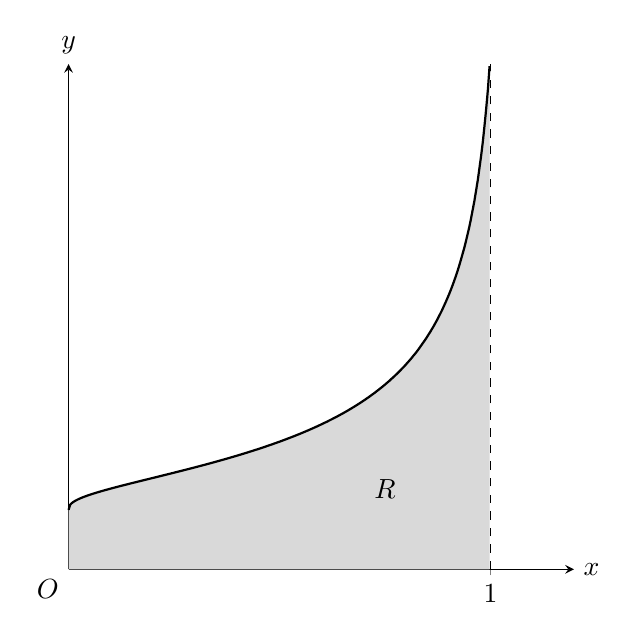
\begin{tikzpicture}
\begin{axis}[
    axis lines=left,
    xlabel={$x$},
    ylabel={$y$},
    xmin=0, xmax=1.15,
    ymin=0, ymax=8.5,
    xtick={0.96},
    xticklabels={$1$},
    ytick=\empty,
    width=8cm,
    height=8cm,
    clip=false,
    every axis x label/.style={at={(ticklabel* cs:1)}, anchor=west},
    every axis y label/.style={at={(ticklabel* cs:1)}, anchor=south}
]
\addplot[draw=none, fill=gray!30, domain=0:0.958, samples=250] {1/sqrt(1 - pow(x,1/3))} \closedcycle;
\addplot[thick, black, domain=0:0.958, samples=250] {1/sqrt(1 - pow(x,1/3))};
\addplot[dashed, black] coordinates {(0.96,0) (0.96,8.5)};
\node[below left] at (axis cs:0,0) {$O$};
\node at (axis cs:0.72,1.35) {$R$};
\end{axis}
\end{tikzpicture}
\end{figure}


The function $f$ is defined by
\[
f(x)=-3\sin\left(5\cos^{-1}\left(x^{\frac{1}{6}}\right)\right)-25\sin\left(3\cos^{-1}\left(x^{\frac{1}{6}}\right)\right)-150\sin\left(\cos^{-1}\left(x^{\frac{1}{6}}\right)\right), \qquad 0\le x<1
\] \\
\begin{enumerate}[label=\textbf{(\alph*)}, resume]
  \item Show that
  \[
  f'(x)=\frac{40}{\sqrt{1-x^{\frac{1}{3}}}}
  \]
  \marks[-20pt]{6}
\end{enumerate}
The diagram shows the curve with equation
\[
y=\frac{1}{\sqrt{1-x^{\frac{1}{3}}}}
\] \\
for $0\le x<1$ and the asymptote $x=1$. The region $R$ is the unbounded region between the curve, the $x$-axis, the line $x=0$ and the line $x=1$. \\
You are given that the area of $R$ is finite. \\
\begin{enumerate}[label=\textbf{(\alph*)}, resume]
  \item Determine the exact area of $R$. \marks{3} \\
\end{enumerate}

\vspace*{10pt}

\begin{tcolorbox}[colback=white, colframe=scarlet, title={\textbf{Solution}}, breakable, grow to left by=6mm, grow to right by=10mm]
\begin{enumerate}[label=\textbf{(\alph*)}]
  \item Let \(c=\cos\theta\) and \(s=\sin\theta\).

  Using de Moivre's theorem,
  \[
  (\cos\theta+\mathrm{i}\sin\theta)^5=\cos 5\theta+\mathrm{i}\sin 5\theta
  \]

  Expanding the left-hand side,
  \begin{align*}
  (c+\mathrm{i}s)^5
  &=c^5+5c^4(\mathrm{i}s)+10c^3(\mathrm{i}s)^2+10c^2(\mathrm{i}s)^3+5c(\mathrm{i}s)^4+(\mathrm{i}s)^5 \\
  &=c^5+5\mathrm{i}c^4s-10c^3s^2-10\mathrm{i}c^2s^3+5cs^4+\mathrm{i}s^5
  \end{align*}

  Taking real parts,
  \[
  \cos 5\theta=c^5-10c^3s^2+5cs^4
  \]

  Since \(s^2=1-c^2\),
  \begin{align*}
  \cos 5\theta
  &=c^5-10c^3(1-c^2)+5c(1-c^2)^2 \\
  &=c^5-10c^3+10c^5+5c(1-2c^2+c^4) \\
  &=16c^5-20c^3+5c
  \end{align*}

  Similarly, from
  \[
  (\cos\theta+\mathrm{i}\sin\theta)^3=\cos 3\theta+\mathrm{i}\sin 3\theta
  \]
  we get
  \begin{align*}
  (c+\mathrm{i}s)^3
  &=c^3+3c^2(\mathrm{i}s)+3c(\mathrm{i}s)^2+(\mathrm{i}s)^3 \\
  &=c^3+3\mathrm{i}c^2s-3cs^2-\mathrm{i}s^3
  \end{align*}
  so taking real parts,
  \begin{align*}
  \cos 3\theta
  &=c^3-3cs^2 \\
  &=c^3-3c(1-c^2) \\
  &=4c^3-3c
  \end{align*}

  Now use
  \[
  c^5\equiv A\cos 5\theta+B\cos 3\theta+C\cos\theta
  \]

  Substituting the expansions,
  \begin{align*}
  c^5
  &\equiv A(16c^5-20c^3+5c)+B(4c^3-3c)+Cc \\
  &\equiv 16Ac^5+(-20A+4B)c^3+(5A-3B+C)c
  \end{align*}

  Equating coefficients of powers of \(c\),
  \begin{align*}
  16A&=1 \\
  -20A+4B&=0 \\
  5A-3B+C&=0
  \end{align*}

  So
  \begin{align*}
  A&=\frac1{16} \\
  -20\left(\frac1{16}\right)+4B&=0 \implies 4B=\frac54 \implies B=\frac5{16} \\
  5\left(\frac1{16}\right)-3\left(\frac5{16}\right)+C&=0 \implies -\frac{10}{16}+C=0 \implies C=\frac{10}{16}=\frac58
  \end{align*}

  Hence
  \[
  A=\frac1{16},\qquad B=\frac5{16},\qquad C=\frac58
  \]

  \item Let
  \[
  \theta=\cos^{-1}\left(x^{1/6}\right)
  \]
  so that
  \[
  \cos\theta=x^{1/6}
  \]

  Then
  \[
  f(x)=-3\sin 5\theta-25\sin 3\theta-150\sin\theta
  \]

  Differentiate using the chain rule:
  \begin{align*}
  f'(x)
  &=-3(5\cos 5\theta)\frac{\mathrm{d}\theta}{\mathrm{d}x}
    -25(3\cos 3\theta)\frac{\mathrm{d}\theta}{\mathrm{d}x}
    -150(\cos\theta)\frac{\mathrm{d}\theta}{\mathrm{d}x} \\
  &=-(15\cos 5\theta+75\cos 3\theta+150\cos\theta)\frac{\mathrm{d}\theta}{\mathrm{d}x}
  \end{align*}

  Now
  \[
  \theta=\cos^{-1}(x^{1/6})
  \]
  and
  \[
  \frac{\mathrm{d}}{\mathrm{d}x}\bigl(\cos^{-1}u\bigr)=-\frac{1}{\sqrt{1-u^2}}\frac{\mathrm{d}u}{\mathrm{d}x}
  \]

  Here \(u=x^{1/6}\), so
  \[
  \frac{\mathrm{d}u}{\mathrm{d}x}=\frac16x^{-5/6}
  \]
  and therefore
  \begin{align*}
  \frac{\mathrm{d}\theta}{\mathrm{d}x}
  &=-\frac{1}{\sqrt{1-(x^{1/6})^2}}\cdot\frac16x^{-5/6} \\
  &=-\frac{x^{-5/6}}{6\sqrt{1-x^{1/3}}}
  \end{align*}

  Substitute this into the expression for \(f'(x)\):
  \begin{align*}
  f'(x)
  &=-(15\cos 5\theta+75\cos 3\theta+150\cos\theta)\left(-\frac{x^{-5/6}}{6\sqrt{1-x^{1/3}}}\right) \\
  &=\frac{x^{-5/6}}{6\sqrt{1-x^{1/3}}}(15\cos 5\theta+75\cos 3\theta+150\cos\theta) \\
  &=\frac{5}{2}\cdot\frac{x^{-5/6}}{\sqrt{1-x^{1/3}}}\bigl(\cos 5\theta+5\cos 3\theta+10\cos\theta\bigr)
  \end{align*}

  From part (a),
  \[
  \cos^5\theta=\frac1{16}\cos 5\theta+\frac5{16}\cos 3\theta+\frac58\cos\theta
  \]

  Multiply by \(16\):
  \[
  16\cos^5\theta=\cos 5\theta+5\cos 3\theta+10\cos\theta
  \]

  So
  \begin{align*}
  f'(x)
  &=\frac{5}{2}\cdot\frac{x^{-5/6}}{\sqrt{1-x^{1/3}}}\cdot 16\cos^5\theta
  \end{align*}

  But \(\cos\theta=x^{1/6}\), so
  \[
  \cos^5\theta=\left(x^{1/6}\right)^5=x^{5/6}
  \]

  Hence
  \begin{align*}
  f'(x)
  &=\frac{5}{2}\cdot\frac{x^{-5/6}}{\sqrt{1-x^{1/3}}}\cdot 16x^{5/6} \\
  &=\frac{40}{\sqrt{1-x^{1/3}}}
  \end{align*}

  Therefore
  \[
  f'(x)=\frac{40}{\sqrt{1-x^{1/3}}}
  \]

  \item The area of \(R\) is
  \[
  \int_0^1 \frac{1}{\sqrt{1-x^{1/3}}}\,\mathrm{d}x
  \]

  Since the curve has asymptote \(x=1\), this is an improper integral:
  \begin{align*}
  \text{Area of }R
  &=\lim_{b\to 1^-}\int_0^b \frac{1}{\sqrt{1-x^{1/3}}}\,\mathrm{d}x
  \end{align*}

  From part (b),
  \[
  \frac{1}{\sqrt{1-x^{1/3}}}=\frac1{40}f'(x)
  \]

  So
  \begin{align*}
  \text{Area of }R
  &=\frac1{40}\lim_{b\to 1^-}\int_0^b f'(x)\,\mathrm{d}x \\
  &=\frac1{40}\lim_{b\to 1^-}\bigl[f(x)\bigr]_0^b \\
  &=\frac1{40}\left(\lim_{b\to 1^-}f(b)-f(0)\right)
  \end{align*}

  First find \(\displaystyle \lim_{b\to 1^-}f(b)\).

  As \(b\to 1^-\),
  \[
  b^{1/6}\to 1
  \qquad\text{so}\qquad
  \cos^{-1}(b^{1/6})\to 0
  \]
  and therefore
  \[
  f(b)\to -3\sin 0-25\sin 0-150\sin 0=0
  \]

  Now find \(f(0)\):
  \[
  \cos^{-1}(0^{1/6})=\cos^{-1}(0)=\frac{\pi}{2}
  \]
  so
  \begin{align*}
  f(0)
  &=-3\sin\left(5\cdot\frac{\pi}{2}\right)-25\sin\left(3\cdot\frac{\pi}{2}\right)-150\sin\left(\frac{\pi}{2}\right) \\
  &=-3(1)-25(-1)-150(1) \\
  &=-3+25-150 \\
  &=-128
  \end{align*}

  Hence
  \begin{align*}
  \text{Area of }R
  &=\frac1{40}\bigl(0-(-128)\bigr) \\
  &=\frac{128}{40} \\
  &=\frac{16}{5}
  \end{align*}

  The exact area of \(R\) is \(\displaystyle \frac{16}{5}\).
\end{enumerate}
\end{tcolorbox}


\newpage

% ---- Question 15 ----
\questionitem

\begin{enumerate}[label=\textbf{(\roman*)}]
  \item Use de Moivre's theorem to show that
  \[
  \cos 5\theta \equiv \cos \theta \left(1 - 12\sin^2 \theta + 16\sin^4 \theta\right)
  \]
  \marks[-20pt]{5}
  \item Hence determine the range of values of
  \[
  \frac{\cos 5\theta}{\cos \theta}
  \]
  given that $\cos \theta \ne 0$. \marks{7} \\
\end{enumerate}

\vspace*{10pt}

\begin{tcolorbox}[colback=white, colframe=scarlet, title={\textbf{Solution}}, breakable, grow to left by=6mm, grow to right by=10mm]
\begin{enumerate}[label=\textbf{(\roman*)}]
  \item Using de Moivre's theorem,
\[
(\cos \theta+\mathrm{i}\sin \theta)^5=\cos 5\theta+\mathrm{i}\sin 5\theta
\]

Expand the left-hand side by the binomial theorem:
\begin{align*}
(\cos \theta+\mathrm{i}\sin \theta)^5
&= \cos^5\theta + 5\cos^4\theta(\mathrm{i}\sin\theta)
+10\cos^3\theta(\mathrm{i}\sin\theta)^2 \\
&\qquad +10\cos^2\theta(\mathrm{i}\sin\theta)^3
+5\cos\theta(\mathrm{i}\sin\theta)^4
+(\mathrm{i}\sin\theta)^5
\end{align*}

Now use
\[
\mathrm{i}^2=-1,\qquad \mathrm{i}^3=-\mathrm{i},\qquad \mathrm{i}^4=1,\qquad \mathrm{i}^5=\mathrm{i}
\]

So
\begin{align*}
(\cos \theta+\mathrm{i}\sin \theta)^5
&= \cos^5\theta + 5\mathrm{i}\cos^4\theta\sin\theta
-10\cos^3\theta\sin^2\theta \\
&\qquad -10\mathrm{i}\cos^2\theta\sin^3\theta
+5\cos\theta\sin^4\theta
+\mathrm{i}\sin^5\theta
\end{align*}

Equating real parts gives
\[
\cos 5\theta=\cos^5\theta-10\cos^3\theta\sin^2\theta+5\cos\theta\sin^4\theta
\]

Factor out $\cos\theta$:
\[
\cos 5\theta=\cos\theta\left(\cos^4\theta-10\cos^2\theta\sin^2\theta+5\sin^4\theta\right)
\]

Now use $\cos^2\theta=1-\sin^2\theta$:
\begin{align*}
\cos 5\theta
&= \cos\theta\left((1-\sin^2\theta)^2-10(1-\sin^2\theta)\sin^2\theta+5\sin^4\theta\right) \\
&= \cos\theta\left(1-2\sin^2\theta+\sin^4\theta-10\sin^2\theta+10\sin^4\theta+5\sin^4\theta\right) \\
&= \cos\theta\left(1-12\sin^2\theta+16\sin^4\theta\right)
\end{align*}

Hence
\[
\cos 5\theta \equiv \cos \theta \left(1 - 12\sin^2 \theta + 16\sin^4 \theta\right)
\]

  \item From part (i),
\[
\frac{\cos 5\theta}{\cos\theta}=1-12\sin^2\theta+16\sin^4\theta
\]
provided $\cos\theta\ne 0$.

Let
\[
u=\sin^2\theta
\]
Then, since $0\le \sin^2\theta \le 1$ and $\cos\theta\ne 0$, we have
\[
0\le u<1
\]

So we need the range of
\[
f(u)=1-12u+16u^2
\qquad \text{for } 0\le u<1
\]

This is a quadratic opening upwards, so its minimum occurs at the vertex:
\[
u=\frac{-(-12)}{2\cdot 16}=\frac{12}{32}=\frac{3}{8}
\]

The minimum value is
\begin{align*}
f\left(\frac38\right)
&=1-12\left(\frac38\right)+16\left(\frac38\right)^2 \\
&=1-\frac{36}{8}+16\cdot \frac{9}{64} \\
&=1-\frac92+\frac94 \\
&=\frac44-\frac{18}{4}+\frac94 \\
&=-\frac54
\end{align*}

So the least possible value is
\[
-\frac54
\]

Now consider the largest possible value on $0\le u<1$.

As $u\to 1^{-}$,
\[
f(u)\to 1-12+16=5
\]

We must check whether $5$ is actually attained. Solve
\begin{align*}
1-12u+16u^2 &= 5 \\
16u^2-12u-4 &= 0 \\
4u^2-3u-1 &= 0 \\
(4u+1)(u-1)&=0
\end{align*}

So
\[
u=1 \quad \text{or} \quad u=-\frac14
\]

But $u=\sin^2\theta$ cannot be negative, and $u=1$ would mean
\[
\sin^2\theta=1 \implies \cos\theta=0
\]
which is excluded.

So $5$ is not attained.

Therefore the range of
\[
\frac{\cos 5\theta}{\cos\theta}
\]
is
\[
-\frac54 \leq \frac{\cos 5\theta}{\cos\theta} < 5
\]

\end{enumerate}
\end{tcolorbox}


\newpage

% ---- Question 16 ----
\questionitem

\begin{enumerate}[label=\textbf{(\alph*)}]
  \item Use de Moivre's theorem to show that
  \[
  \cos 5\theta = 16\cos^5 \theta - 20\cos^3 \theta + 5\cos \theta
  \]
  \marks[-20pt]{5}
  \item Use the identity given in part (a) to find the $2$ positive roots of
  \[
  64x^5 - 80x^3 + 20x + 1 = 0
  \]
  giving your answers to $3$ significant figures. \marks{4} \\
\end{enumerate}

\vspace*{10pt}

\begin{tcolorbox}[colback=white, colframe=scarlet, title={\textbf{Solution}}, breakable, grow to left by=6mm, grow to right by=10mm]
\begin{enumerate}[label=\textbf{(\alph*)}]
  \item Let \(c=\cos\theta\) and \(s=\sin\theta\). By de Moivre's theorem,
\[
(c+\mathrm{i}s)^5=\cos5\theta+\mathrm{i}\sin5\theta
\]
Expanding the left-hand side,
\begin{align*}
(c+\mathrm{i}s)^5
&=c^5+5c^4(\mathrm{i}s)+10c^3(\mathrm{i}s)^2+10c^2(\mathrm{i}s)^3+5c(\mathrm{i}s)^4+(\mathrm{i}s)^5\\
&=c^5+5\mathrm{i}c^4s-10c^3s^2-10\mathrm{i}c^2s^3+5cs^4+\mathrm{i}s^5
\end{align*}
Equating real parts gives
\[
\cos5\theta=c^5-10c^3s^2+5cs^4
\]
Now use \(s^2=1-c^2\) and \(s^4=(1-c^2)^2\):
\begin{align*}
\cos5\theta
&=c^5-10c^3(1-c^2)+5c(1-c^2)^2\\
&=c^5-10c^3+10c^5+5c(1-2c^2+c^4)\\
&=c^5-10c^3+10c^5+5c-10c^3+5c^5\\
&=16c^5-20c^3+5c
\end{align*}
Since \(c=\cos\theta\),
\[
\cos5\theta=16\cos^5\theta-20\cos^3\theta+5\cos\theta
\]
as required.

  \item Let
\[
x=\cos\theta \qquad \text{with } 0^\circ\le \theta \le 180^\circ
\]
Then
\begin{align*}
64x^5-80x^3+20x+1&=0\\
4(16x^5-20x^3+5x)+1&=0
\end{align*}
Using the identity from part (a),
\[
16x^5-20x^3+5x=\cos5\theta
\]
so
\[
4\cos5\theta+1=0
\]
Hence
\[
\cos5\theta=-\frac14
\]
Let
\[
\alpha=\arccos\!\left(-\frac14\right)\approx 104.478^\circ
\]
Since \(0^\circ\le \theta \le 180^\circ\), we have \(0^\circ\le 5\theta \le 900^\circ\). Therefore the solutions for \(5\theta\) in this interval are
\[
\alpha,\quad 360^\circ-\alpha,\quad 360^\circ+\alpha,\quad 720^\circ-\alpha,\quad 720^\circ+\alpha
\]
So
\[
\theta\approx 20.896^\circ,\ 51.104^\circ,\ 92.896^\circ,\ 123.104^\circ,\ 164.896^\circ
\]
Now \(x=\cos\theta\), and \(x>0\) when \(0^\circ<\theta<90^\circ\). So only the first two values give positive roots:
\begin{align*}
x&=\cos20.896^\circ\approx 0.934\\
x&=\cos51.104^\circ\approx 0.628
\end{align*}
So the two positive roots are \(x\approx 0.628\) and \(x\approx 0.934\).
\end{enumerate}
\end{tcolorbox}


\newpage

% ---- Question 17 ----
\questionitem

\begin{enumerate}[label=\textbf{(\alph*)}]
  \item Use de Moivre’s theorem to show that
  \[
  \sin^2 \theta \cos^2 \theta = \frac{1}{8}(1-\cos 4\theta)
  \]
  \marks[-20pt]{5}
  \item Hence, or otherwise, find the solution of the differential equation
  \[
  \frac{\mathrm{d}y}{\mathrm{d}\theta} - 2y\tan \theta = \sin^2 \theta
  \]
  for which $y=0$ when $\theta=\frac{1}{4}\pi$. \marks{6} \\
\end{enumerate}

\vspace*{10pt}

\begin{tcolorbox}[colback=white, colframe=scarlet, title={\textbf{Solution}}, breakable, grow to left by=6mm, grow to right by=10mm]
\begin{enumerate}[label=\textbf{(\alph*)}]
  \item By de Moivre's theorem,
\[
(\cos\theta+\mathrm{i}\sin\theta)^4=\cos4\theta+\mathrm{i}\sin4\theta
\]

Expanding the left-hand side,
\[
\begin{aligned}
(\cos\theta+\mathrm{i}\sin\theta)^4
&=\cos^4\theta+4\cos^3\theta(\mathrm{i}\sin\theta)+6\cos^2\theta(\mathrm{i}\sin\theta)^2 \\
&\qquad +4\cos\theta(\mathrm{i}\sin\theta)^3+(\mathrm{i}\sin\theta)^4 \\
&=\cos^4\theta+4\mathrm{i}\cos^3\theta\sin\theta-6\cos^2\theta\sin^2\theta \\
&\qquad -4\mathrm{i}\cos\theta\sin^3\theta+\sin^4\theta
\end{aligned}
\]

So, comparing real parts,
\[
\cos4\theta=\cos^4\theta-6\sin^2\theta\cos^2\theta+\sin^4\theta
\]

Now rewrite the right-hand side as
\[
\begin{aligned}
\cos^4\theta-6\sin^2\theta\cos^2\theta+\sin^4\theta
&=(\sin^2\theta+\cos^2\theta)^2-8\sin^2\theta\cos^2\theta \\
&=1-8\sin^2\theta\cos^2\theta
\end{aligned}
\]

Hence
\[
\cos4\theta=1-8\sin^2\theta\cos^2\theta
\]

Therefore,
\[
\sin^2\theta\cos^2\theta=\frac{1-\cos4\theta}{8}
\]

So
\[
\sin^2\theta\cos^2\theta=\frac{1}{8}(1-\cos4\theta)
\]

  \item The differential equation is
\[
\frac{\mathrm{d}y}{\mathrm{d}\theta}-2y\tan\theta=\sin^2\theta
\]

This is a linear first order differential equation of the form
\[
\frac{\mathrm{d}y}{\mathrm{d}\theta}+P(\theta)y=Q(\theta)
\]
with
\[
P(\theta)=-2\tan\theta
\]

The integrating factor is
\[
\mu(\theta)=e^{\int -2\tan\theta\,\mathrm{d}\theta}
\]

Using
\[
\int \tan\theta\,\mathrm{d}\theta=-\ln|\cos\theta|
\]
we get
\[
\mu(\theta)=e^{2\ln|\cos\theta|}=\cos^2\theta
\]

Multiply the differential equation through by \(\cos^2\theta\):
\[
\cos^2\theta\frac{\mathrm{d}y}{\mathrm{d}\theta}-2y\sin\theta\cos\theta=\sin^2\theta\cos^2\theta
\]

The left-hand side is
\[
\frac{\mathrm{d}}{\mathrm{d}\theta}(y\cos^2\theta)
\]

So
\[
\frac{\mathrm{d}}{\mathrm{d}\theta}(y\cos^2\theta)=\sin^2\theta\cos^2\theta
\]

Using part (a),
\[
\frac{\mathrm{d}}{\mathrm{d}\theta}(y\cos^2\theta)=\frac{1-\cos4\theta}{8}
\]

Integrating,
\[
\begin{aligned}
y\cos^2\theta
&=\int \frac{1-\cos4\theta}{8}\,\mathrm{d}\theta \\
&=\frac{1}{8}\int 1\,\mathrm{d}\theta-\frac{1}{8}\int \cos4\theta\,\mathrm{d}\theta \\
&=\frac{\theta}{8}-\frac{\sin4\theta}{32}+C
\end{aligned}
\]

Now use the condition \(y=0\) when \(\theta=\frac{\pi}{4}\):
\[
0\cdot \cos^2\frac{\pi}{4}=\frac{1}{8}\cdot\frac{\pi}{4}-\frac{\sin\pi}{32}+C
\]

So
\[
0=\frac{\pi}{32}+C
\]
and hence
\[
C=-\frac{\pi}{32}
\]

Therefore,
\[
y\cos^2\theta=\frac{\theta}{8}-\frac{\sin4\theta}{32}-\frac{\pi}{32}
\]

So
\[
y=\frac{\frac{4\theta}{32}-\frac{\sin4\theta}{32}-\frac{\pi}{32}}{\cos^2\theta}
=\frac{4\theta-\sin4\theta-\pi}{32\cos^2\theta}
\]

Thus the required solution is
\[
y=\frac{4\theta-\sin4\theta-\pi}{32\cos^2\theta}
\]
  \end{enumerate}
\end{tcolorbox}


\newpage

% ---- Question 18 ----
\questionitem

\begin{enumerate}[label=\textbf{(\alph*)}]
  \item Use de Moivre’s theorem to show that
  \[
  \cos^6 \theta = a \cos 6\theta + b \cos 4\theta + c \cos 2\theta + d
  \]
  where $a$, $b$, $c$ and $d$ are constants to be found. \marks{5} \\
  \item Hence show that
  \[
  \int_0^{\pi/4} \cos^6 \theta \, \mathrm{d}\theta = \frac{11}{48} + \frac{5\pi}{64}
  \]
  \marks[-30pt]{5}
\end{enumerate}

\vspace*{10pt}

\begin{tcolorbox}[colback=white, colframe=scarlet, title={\textbf{Solution}}, breakable, grow to left by=6mm, grow to right by=10mm]
\begin{enumerate}[label=\textbf{(\alph*)}]
  \item Let
  \[
  z=e^{\mathrm{i}\theta}
  \]
  Then
  \[
  \cos\theta=\frac{z+z^{-1}}{2}
  \]
  and, by de Moivre's theorem,
  \[
  z^n+z^{-n}=e^{\mathrm{i}n\theta}+e^{-\mathrm{i}n\theta}=2\cos n\theta
  \]

  Now
  \[
  64\cos^6\theta=(z+z^{-1})^6
  \]

  Expanding by the binomial theorem,
  \begin{align*}
  (z+z^{-1})^6
  &=z^6+6z^4+15z^2+20+15z^{-2}+6z^{-4}+z^{-6}
  \end{align*}

  Group the terms in pairs:
  \begin{align*}
  64\cos^6\theta
  &=(z^6+z^{-6})+6(z^4+z^{-4})+15(z^2+z^{-2})+20 \\
  &=2\cos 6\theta+12\cos 4\theta+30\cos 2\theta+20
  \end{align*}

  Dividing by \(64\),
  \begin{align*}
  \cos^6\theta
  &=\frac{1}{32}\cos 6\theta+\frac{12}{64}\cos 4\theta+\frac{30}{64}\cos 2\theta+\frac{20}{64} \\
  &=\frac{1}{32}\cos 6\theta+\frac{3}{16}\cos 4\theta+\frac{15}{32}\cos 2\theta+\frac{5}{16}
  \end{align*}

  Hence
  \[
  a=\frac{1}{32},\qquad b=\frac{3}{16},\qquad c=\frac{15}{32},\qquad d=\frac{5}{16}
  \]

  \item Using the identity from part (a),
  \[
  \cos^6\theta=\frac{1}{32}\bigl(\cos 6\theta+6\cos 4\theta+15\cos 2\theta+10\bigr)
  \]

  So
  \begin{align*}
  \int_0^{\pi/4}\cos^6\theta\,\mathrm{d}\theta
  &=\frac{1}{32}\int_0^{\pi/4}\bigl(\cos 6\theta+6\cos 4\theta+15\cos 2\theta+10\bigr)\,\mathrm{d}\theta \\
  &=\frac{1}{32}\left[\frac{1}{6}\sin 6\theta+\frac{6}{4}\sin 4\theta+\frac{15}{2}\sin 2\theta+10\theta\right]_0^{\pi/4} \\
  &=\frac{1}{32}\left[\frac{1}{6}\sin 6\theta+\frac{3}{2}\sin 4\theta+\frac{15}{2}\sin 2\theta+10\theta\right]_0^{\pi/4}
  \end{align*}

  At \(\theta=\frac{\pi}{4}\),
  \[
  \sin\frac{3\pi}{2}=-1,\qquad \sin\pi=0,\qquad \sin\frac{\pi}{2}=1
  \]

  Therefore
  \begin{align*}
  \int_0^{\pi/4}\cos^6\theta\,\mathrm{d}\theta
  &=\frac{1}{32}\left(-\frac{1}{6}+\frac{3}{2}\cdot 0+\frac{15}{2}\cdot 1+10\cdot \frac{\pi}{4}\right) \\
  &=\frac{1}{32}\left(-\frac{1}{6}+\frac{15}{2}+\frac{5\pi}{2}\right) \\
  &=\frac{1}{32}\left(\frac{44}{6}+\frac{5\pi}{2}\right) \\
  &=\frac{11}{48}+\frac{5\pi}{64}
  \end{align*}

  Hence
  \[
  \int_0^{\pi/4}\cos^6\theta\,\mathrm{d}\theta=\frac{11}{48}+\frac{5\pi}{64}
  \]
\end{enumerate}
\end{tcolorbox}


\end{enumerate}
\end{document}
